We now review the protocol presented in \cite{giordani2020} which utilises quantum walk dynamics in order to generate higher dimensional entanglement.

The imagined setup of this protocol is that there are two labs, $A$ and $B$, which have a shared source of entangled qubits but are otherwise spatially separated and cannot interact with one another.

In this section we use following notation:
\begin{itemize}
    \item $\ket{u}_J$ is a state belonging to the subspace $\mathcal{H}_J = \mathcal{H}^{(A)}_J \otimes \mathcal{H}^{(B)}_J, J\in\{C,W\}$.
    \item $\ket{u}^{(K)}$ is a state belonging to the subspace $\mathcal{H}^{(K)} = \mathcal{H}^{(K)}_C \otimes \mathcal{H}^{(K)}_W, K\in\{A,B\}$.
    \item  $\ket{u}^{(K)}_J$ is a state belonging to the subspace $\mathcal{H}^{(K)}_J$.
\end{itemize}

In this mathematical framework the overall Hilbert space of the quantum system is comprised of two quantum walk subspaces,
\begin{align}
    \mathcal{H} &= \mathcal{H}^{(A)} \otimes \mathcal{H}^{(B)}\\
                &= \mathcal{H}^{(A)}_C \otimes \mathcal{H}^{(A)}_W \otimes \mathcal{H}^{(B)}_C \otimes \mathcal{H}^{(B)}_W.
\end{align}

The basic premise of this protocol is this:
\begin{enumerate}
    \item Entangle the two coin spaces of the walkers $\mathcal{H}^{(K)}_C$. (Fig \ref{fig:preparation}.)
    \item Proceed with the quantum walk for some determined number of steps.
    \item Use a projection $\mathcal{P}_\gamma = \ket{\gamma}\bra{\gamma}, \ket{\gamma}\in\mathcal{H}^{(A)}_C$ to then transfer the entanglement so that it solely exists in the subspace $\mathcal{H}^{(A)}_W \otimes \mathcal{H}^{(B)}_C \otimes \mathcal{H}^{(B)}_W$.
    \item In similar fashion, find a projection $\mathcal{P}_\delta = \ket{\delta}\bra{\delta}, \ket{\delta}\in\mathcal{H}^{(B)}_C$ to transfer the entanglement to exist between the two walker subspaces, $\mathcal{H}^{(i)}_W$, only.
    \item Accumulate entanglement in the walker subspaces by once more entangling the two coin spaces and repeating the protocol.
\end{enumerate}

\begin{figure}
    \centering
    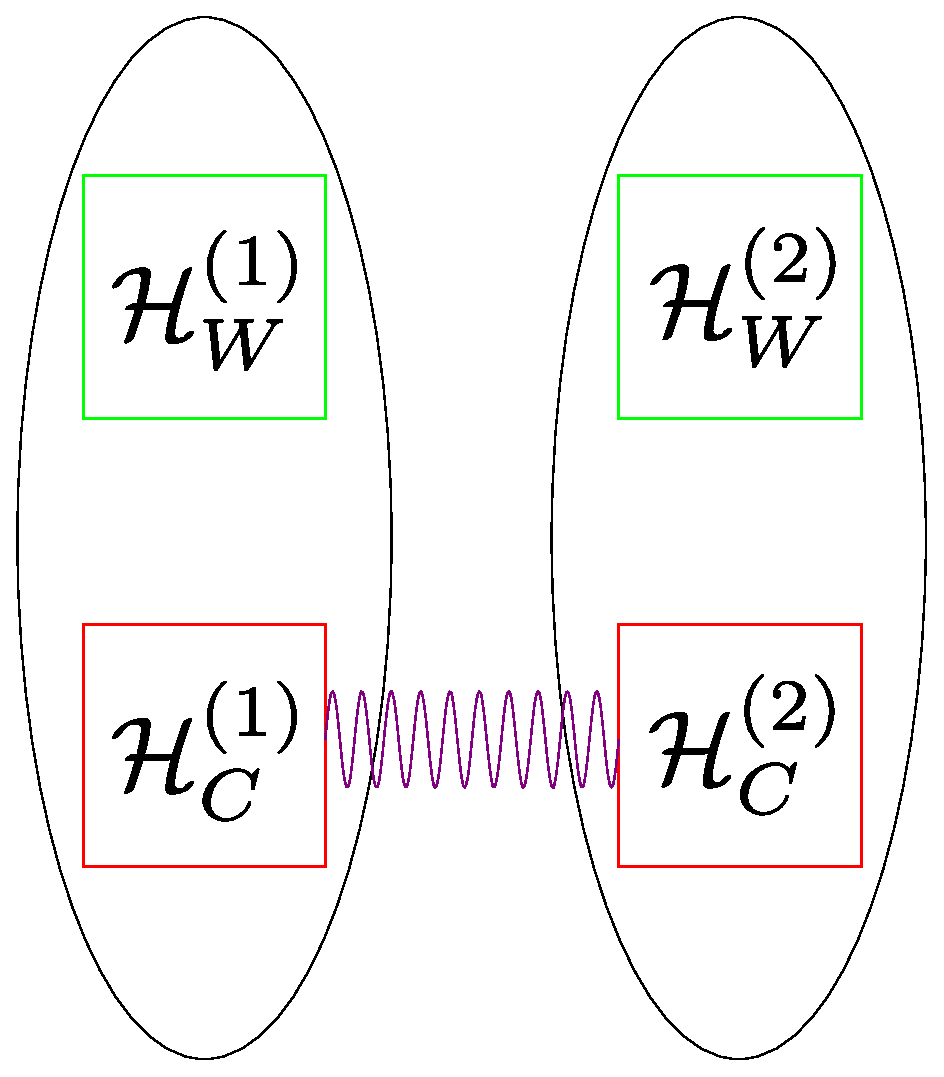
\includegraphics[scale = .25]{preparation}
    \caption{The initial prepared state has entanglement solely between the two coin subspaces. Figure is an edited version from FIG 3 from \cite{giordani2020}.}
    \label{fig:preparation}
\end{figure}

In this way, we are able to generate arbitrary amounts of higher dimensional entanglement.
As is the case with many quantum walk based protocols, particular attention must be paid to the choice of coin used for the quantum walk, as it will have a large impact on the outcomes of the protocol.
The shift operator used in this protocol is the $\tilde{S}$, as outlined in Section \ref{subsection:qw}.

\subsection{Transfer using identity coin operator}
\label{subsection:qw_transfer}
To illustrate the basic principles of the protocol, consider the case where our coin is the identity $I$. A state $\ket{\psi(0)}$ is prepared with the coin states entangled and walkers at the origin
\begin{equation}
    \ket{\psi(0)} = \underbrace{\frac{1}{\sqrt{2}}\Big [\ket{\uparrow}^{(A)}_C\ket{\uparrow}^{(B)}_C + \ket{\downarrow}^{(A)}_C\ket{\downarrow}^{(B)}_C \Big]}_{\text{Bell State}}\otimes \ket{0}^{(A)}_W\ket{0}^{(B)}_W.
\end{equation}
Following this, the "coin", $I$, is applied and then use our shift operator $\tilde{S}$ to advance the quantum walk. Explicitly (dropping the indices and combining some of our kets together) we obtain
\begin{equation}
    \ket{\psi(1)} = \tilde{S}I\ket{\psi} = \frac{1}{\sqrt{2}}\Big [\ket{\uparrow,\uparrow}\ket{0,0} + \ket{\downarrow,\downarrow}\ket{1,1}\Big].
\end{equation}
We then project the part of $\ket{\psi(1)}$ residing in the $\mathcal{H}^{(A)}_C$ subspace onto the vector $\ket{\gamma}$, using the projective operator $\mathcal{P}_\gamma = \ket{\gamma}\bra{\gamma} \in \mathcal{H}^{(A)}_C$. Choose $\ket{\gamma} = \frac{1}{\sqrt{2}} \big [\ket{\uparrow} + \ket{\downarrow} \big]$ which then gives us
\begin{equation}
    \mathcal{P}_\gamma \ket{\psi(1)} = \frac{1}{2}\Big [\ket{\gamma}\otimes \big (\ket{\uparrow, 0, 0} + \ket{\downarrow, 1, 1}\big )\Big ].
\end{equation}
Similarly, we project the other walker subspace to $\ket{\delta}$ which we can in this instance take to be the same state as $\ket{\gamma} = \frac{1}{\sqrt{2}} \big [\ket{\uparrow} + \ket{\downarrow} \big]$,
\begin{equation}
    \mathcal{P}_\delta \mathcal{P}_\gamma \ket{\psi(1)} = \frac{1}{2\sqrt{2}}\Big [\ket{\gamma}\otimes \ket{\delta} \otimes \frac{1}{\sqrt{2}}\Big (\ket{0, 0} + \ket{1, 1}\Big )\Big ].
\end{equation}
Renormalising we see that we have the state
\begin{equation}
    \label{eq:qw_transfer_1_final}
    \ket{\gamma}^{(A)}_C \otimes \ket{\delta}^{(B)}_C \otimes \underbrace{\frac{1}{\sqrt{2}}\Big [\ket{0, 0} + \ket{1, 1}\Big ]_W}_{\text{Bell State}},
\end{equation}
which has a Bell State in the $\mathcal{H}_W$ subspace, and the states in $\mathcal{H}_C$ are separable. Therefore we have transferred the entanglement that originally resided in the coin subspace to the walker one.

\subsection{Accumulation}
\label{subsection:qw_accumulation}
The true motivation behind this protocol, as previously stated, is the ability to accumulate the entanglement transferred from the lower dimensional coin subspace to the higher dimensional walker one. Again, using $I$ as our coin, start with the final state obtained from the first iteration of the protocol (Equation \ref{eq:qw_transfer_1_final}) and re-entangle the coin subspaces, obtaining a new initial state, $\ket{\psi(0)}$
\begin{alignat}{3}
    \ket{\gamma}^{(A)}_C \otimes \ket{\delta}^{(B)}_C&\otimes \frac{1}{\sqrt{2}}\Big [\ket{0, 0} + \ket{1, 1}\Big ]_W\\
    \overset{\text{Entangle }\mathcal{H}_C}{\longrightarrow} \frac{1}{\sqrt{2}} \Big [\ket{\uparrow, \uparrow} + \ket{\downarrow, \downarrow}\Big ]_C&\otimes \frac{1}{\sqrt{2}}\Big [\ket{0, 0} + \ket{1, 1}\Big ]_W\\
    & &:=\ket{\psi(0)}.
\end{alignat}
We then proceed with the walk, however taking two steps instead of one this time,
\begin{align}
    \ket{\psi(2)} &= (\tilde{S}I)^2\ket{\psi(0)}\\
    &= \frac{1}{2}\Big[\ket{\uparrow,\uparrow}\big (\ket{0,0}+\ket{1,1}\big ) + \ket{\downarrow,\downarrow}\big (\ket{2,2} + \ket{3,3}\big )\Big ].
\end{align}
Using the same projection operators in the two coin subspaces, $\mathcal{P}_\gamma \in \mathcal{H}^{(A)}_C,  \mathcal{P}_\delta \in \mathcal{H}^{(B)}_C$, and renormalising gives the final state
\begin{equation}
    \ket{\gamma}\otimes\ket{\delta}\otimes\frac{1}{2}\Big[\ket{0,0} + \ket{1,1} + \ket{2,2} + \ket{3,3}\Big ].
\end{equation}

If we measure the entanglement in the state
\begin{equation}
    \frac{1}{2}\Big[\ket{0,0} + \ket{1,1} + \ket{2,2} + \ket{3,3}\Big ]
\end{equation}
using the log negativity, we find that we have now accumulated two ebits in the walker subspace as desired.
We can continue to repeat this process to accumulate arbitrarily large amounts of entanglement into our walker subspace. The number of steps needed for each iteration of the quantum walk is given as follows.
\begin{claim}
\label{claim:min_steps}
The $n^{th}$ iteration (counting from 1) of the protocol requires at least $2^{n-1}$ steps in the quantum walk.
\end{claim}
\begin{proof}
Each step in a quantum walk with shift operator $\tilde{S}$ increases the number of basis states with non-zero amplitude by 1, provided that the amplitude $\ket{\downarrow}$ coin basis state is non-zero.
Therefore the dimension of each walker can be taken to be $s + 1$, where $s$ is the total number of steps taken in the walk, since the walker space can be reduced to the subspace spanned by the $s+1$ non-zero amplitude basis states.
Using Claim \ref{claim:maximally_entangled_states}, the upper bound on the entanglement that can be held between the two walker states is given by $\log_2(s+1)$ ebits.
This implies the following condition on the total number of steps
\begin{equation}
    \log_2(s+1) \geq n \implies s\geq 2^n -1.
\end{equation}
Assuming that this inequality is satisfied at equality for the $n-1^{th}$ iteration of the protocol gives a total step number of $2^{n-1} -1$.
Therefore, the minimum number of steps for the $n^{th}$ iteration is given by
\begin{align}
    2^{n} - 1 - (2^{n-1} -1) &= 2^n - 2^{n-1}\\
    &= 2 \times 2^{n-1} - 2^{n-1}\\
    &= 2^{n-1}.
\end{align}
\end{proof}
\subsection{Retrieval}
\label{subsection:qw_retrieval}
Although accumulating the entanglement in higher dimensions is of significant use, it is also possible to imagine that we might wish to retrieve the entangled Bell pairs back from our qudits.
For example, consider the case where the method of generating entangled qubits is not deterministic but we have a protocol which requires a large number of Bell pairs to be used at the same time.
If this protocol can be reversed to get Bell pairs back out, then we could store the entangled Bell pairs when they are successfully generated and then retrieve them all at once to ensure we have an adequate number of Bell pairs.
In the case of the identity coin example, it is rather simple to use a near identical setup, where the qudits play the role of the coins and the qubit play the role of the walker, to retrive entangled Bell pairs out of the qudits.
For a general coin, it is also possible in principle to retrieve the entanglement back out of the entangled qudits.
However, retrieval after more than 1 ebit has been transferred for the non-identity coin is not simple within the framework of a quantum walk based protocol, due to the non maximal nature of the entanglement present in the qudits.

\subsection{Drawbacks}
In the example given above, I have demonstrated that this protocol can transfer all of the entanglement to our qudits.
However, this is with the significant caveat that the example does not use quantum walk dynamics in order to transfer the entanglement, as using the identity as a coin is akin to having no coin at all.
In analysing the protocol with the Hadamard coin, it is only possible to transfer one ebit of entanglement optimally, after the first iteration. Subsequent iterations result in loss of entanglement.
Simulations of the protocol for storing two Bell states, equivalent to two ebits, found that at most around 1.6 ebits of entanglement can be stored with a Hadamard QW, as shown in Figure \ref{fig:2ebittransfer}.
Furthermore, the projective measurements employed as part of the protocol mean that it is not unitary and is non trivial to reverse in order to retrieve the entanglement out from the entangled qudits.
The experimental implementation suggested in the paper also required the use of post selection, where undesirable states were discarded and the protocol run again.
All this in combination results in a protocol which is rather inefficient in achieving its aims, and serves more as a proof of concept in that it is possible to use quantum walk dynamics to transfer entanglement, but falls short in being a suitable implementation for the task.

\begin{figure}
    \centering
    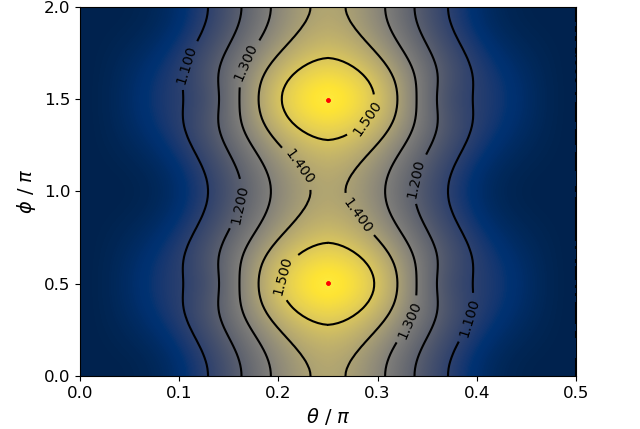
\includegraphics[scale=0.75]{2ebit_transfer.png}
    \caption{Transferring two ebits using the quantum walk protocol proposed by \cite{giordani2020}. $\theta, \phi$ are the parameters describing $\ket{\gamma}$ that defines the projection operator $\mathcal{P}_\gamma$.}
    \label{fig:2ebittransfer}
\end{figure}

However, the example with the identity coin clearly shows that it is possible to efficiently transfer entanglement into qudits, but highlights that an alternative computational model is likely better suited in implementing the ideas proposed.
In Section \ref{section:aqc_transfer}, an alternative protocol in the ancilla-based quantum computing model is proposed which solves the inefficiencies present in this QW based proposal.